\documentclass[12pt,a4paper]{article}
\usepackage{tabularx}
\usepackage[utf8]{inputenc}
\usepackage[catalan]{babel}
\usepackage{amsmath}
\usepackage{amsfonts}
\usepackage{amssymb}
\usepackage{graphicx}
\usepackage{mathtools}
\usepackage{amsfonts}
\usepackage{subcaption}
\usepackage[linktocpage]{hyperref}

\usepackage[bottom]{footmisc}
\usepackage{float}
%\usepackage{cite}
\usepackage{commath}
%code insert
\usepackage{listings}
\usepackage[framed,numbered,autolinebreaks,useliterate]{mcode}
%pict insert
\usepackage{graphicx}
\usepackage[export]{adjustbox}
%
\usepackage[left=2cm,right=2cm,top=2cm,bottom=2cm]{geometry}
\everymath{\displaystyle}
\author{Eva María Urbano González, Pol Fontanes, Boyan Naydenov}
\title{Disseny d'un compressor}

\renewcommand\lstlistingname{Codis}
\renewcommand\lstlistlistingname{Codis}

\begin{document}
\begin{titlepage}
	\centering
	\vspace{4.5cm}
	{\scshape ESEIAAT \par}
	{\scshape\Large Sistemes de Propulsió d'Aeronaus \par}
	\vspace{1.5cm}
	{\huge\bfseries Disseny d'un compressor \par}
	\vspace{15cm}
	{\Large\itshape Eva María Urbano González\par}
	{\Large\itshape Pol Fontanes\par}
	{\Large\itshape Boyan Naydenov\par}
	\vfill
	\vspace{1cm}
	\today
\end{titlepage}
\tableofcontents
\lstlistoflistings
\listoffigures
\pagebreak
\section{Introducció i Objectius}
El present treball forma part de l'assignatura de Sistemes de Propulsió d'Aeronaus. Gran part d'aquesta assignatura consisteix en l'estudi dels tipus de motors d'una aeronau i de les possibilitats d'optimització, a més de la parametrització dels motors tant en cas ideal com en cas real.\\
Per tal de duu a terme un estudi més profund de les àrees de coneixement relacionades amb l'assignatura es proposa la realització d'aquest treball. L'objectiu es el disseny preliminar de la motorització d'un avió. Només es donen tres condicions de disseny, de manera que el sistema no queda definit, si no que s'han d'establir certs criteris per a aconseguir tots els paràmetres del motor. En les següents pàgines es discutirà quin tipus de motor pot ser adequat i el criteri de disseny a utilitzar. Seguidament s'implementarà aquest criteri per obtenir alguns dels paràmetres del avió i després es calcularà la resta tenint en compte que el motor es real. Un cop obtinguda la parametrització, s'afegirà al motor un mixer i un postcombustor. En cas que s'hagi decidit afegir un fan, es seleccionarà l'hèlix. Posteriorment, i un cop obtingut els flux màssic tant d'aire com de combustible, es calcularan les àrees del motor.
\section{Càlcul del primer esglaó del compressor}
Per tal de fer el càlcul del primer esglaó es consideraran diversos valors típics de solidesa i de flux. Amb aquests valors es calcularan els paràmetres necessaris per obtenir el rendiment i el treball per esglaó per a tots els casos. Un cop es tinguin aquests valors, es calcularà el treball necessari per esglaó considerant el treball total a assolir i el número més típic d'esglaons en compressors, trobant així una solució possible i òptima. 
Els valors de solidesa i flux que s'han considerat son:

\begin{equation}
\nonumber \frac{1}{\sigma}=[0.4; 0.6; 0.8; 1.0; 1.2]
\end{equation}
 
\begin{equation}
\nonumber \Psi=[0.4;0.5;0.6;0.7;0.8]
\end{equation}
\subsection{Càlcul de $\beta_a$ i $\beta_b$ en funció de $S/C$ i $\Psi$}
Per a calcular els angles que forma la corrent del flux amb l'eix del rotor, s'utilitzarà el criteri experimental de \textit{Howell} i les hipòtesis mencionades a l'apartat \ref{Intro}. S'obtenen tres equacions amb tres incògnites: $\beta_a$, $\beta_b$ i $\beta_m$: 
\begin{equation}
\tan(\beta_a)-\tan(\beta_b)=\frac{1.55}{1+1.55\frac{S}{C}}
\end{equation} 
\begin{equation}
\tan(\beta_m)=\frac{\tan(\beta_a)+\tan(\beta_b)}{2}
\end{equation}
\begin{equation}
\tan(\beta_m)=\frac{1}{2\Psi}
\end{equation}
Les incògnites es poden aïllar fàcilment per a poder resoldre el sistema. En les següents figures es mostren els resultats per a $\beta_a$ i $\beta_b$. $beta_m$ serà utilitzada per a càlculs posteriors.
\begin{figure}[H]
	\centering
	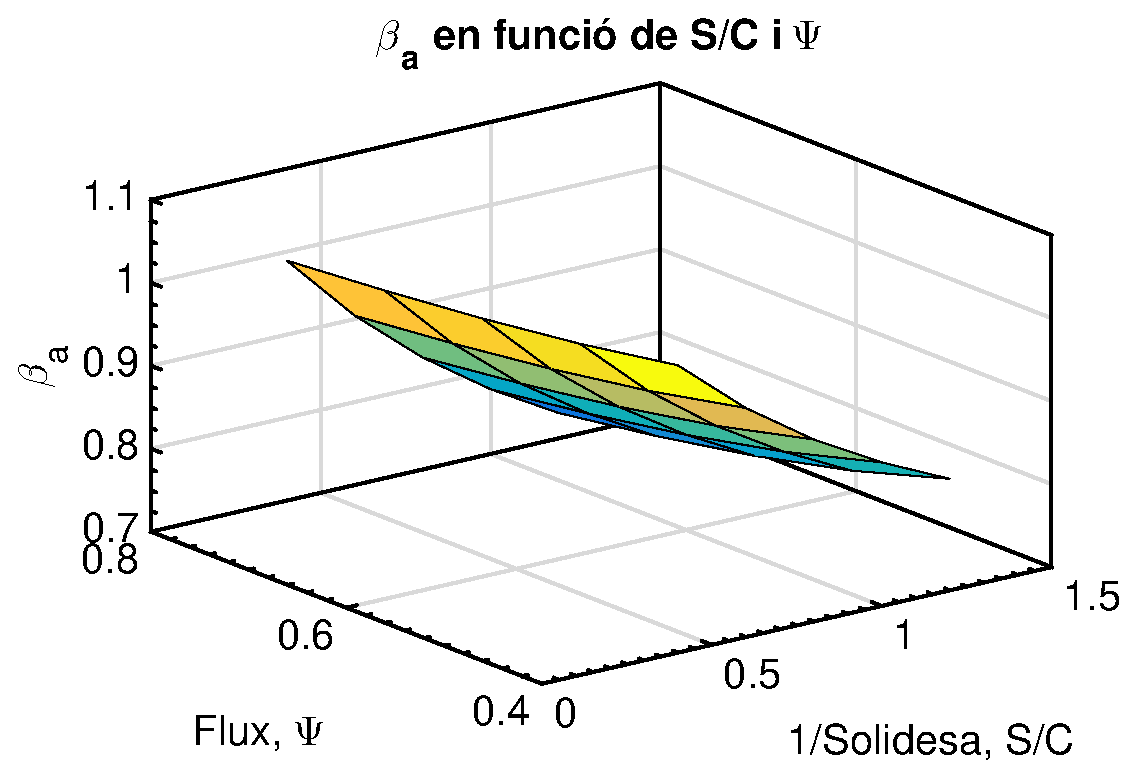
\includegraphics[width=0.8\textwidth]{./code/figures/parametres/betA}
	\caption{Valors de $\beta_a$ en funció de $S/C$ i $\Psi$.}
	\label{betA}
\end{figure}

\begin{figure}[H]
	\centering
	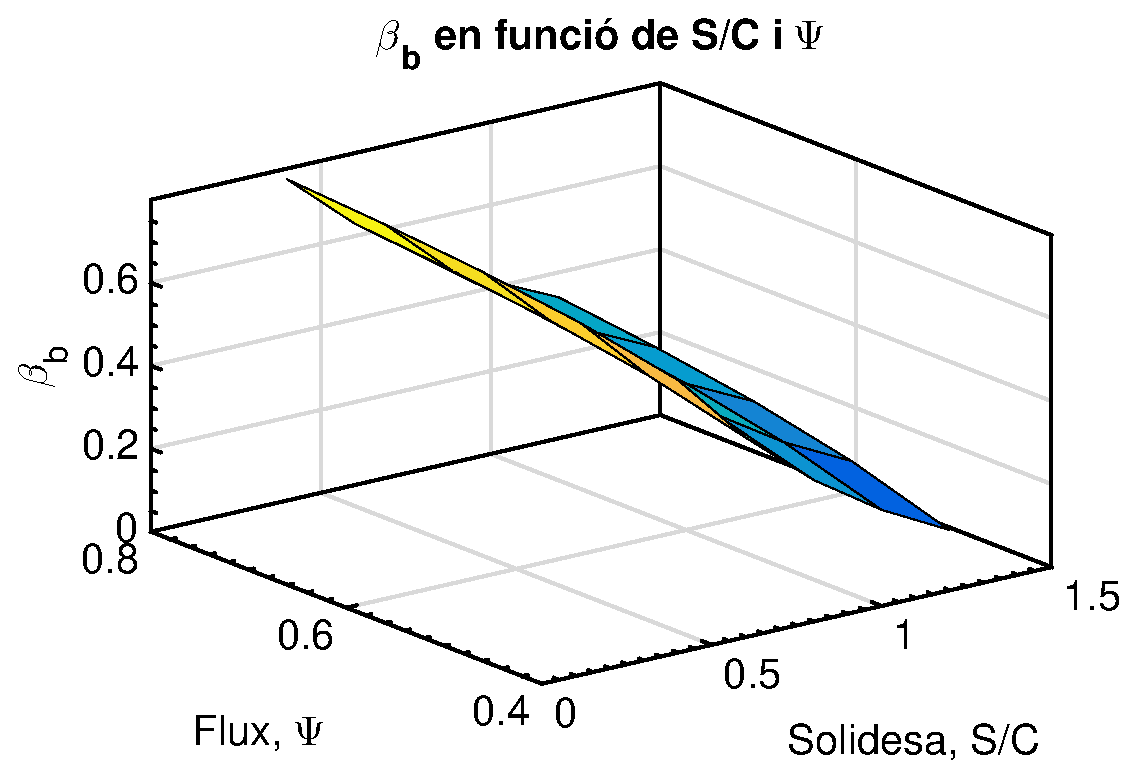
\includegraphics[width=0.8\textwidth]{./code/figures/parametres/betB}
	\caption{Valors de $\beta_b$ en funció de $S/C$ i $\Psi$.}
	\label{betB}
\end{figure}

\subsection{Càlcul de $C_D$ i $C_L$ en funció de $S/C$ i $\Psi$}
Les expressions per a calcular la sustentació i la resistència han sigut obtingudes analitzant el volum de control enter dos àleps. Se suposa que el procés que té lloc es estacionari i que el flux es incompressible. Es realitza un anàlisi utilitzant les equacions de la quantitat de moviment per obtenir la força en la direcció axial i en la direcció angular. A partir d'aquestes equacions, la sustentació i la resistència es poden calcular com: 
\begin{equation}
L= F_\theta \cos\beta_m+F_z \sin\beta_m
\end{equation}
\begin{equation}
D= F_\theta \sin\beta_m-F_z \cos\beta_m
\end{equation}
Substituint expressions i adimensionalitzant s'obté: 
\begin{equation}
C_L=2\frac{S}{C}(\tan\beta_a-\tan\beta_b)\cos\beta_m-C_D\tan\beta_m
\end{equation} 
\begin{equation}
C_D=0.021+\frac{0.02}{2.5}\frac{S}{C}+0.018C_L^2
\end{equation}
Que es un sistema de dues equacions amb dues incògnites. Els resultats es mostren en les següents figures.

\begin{figure}[H]
	\centering
	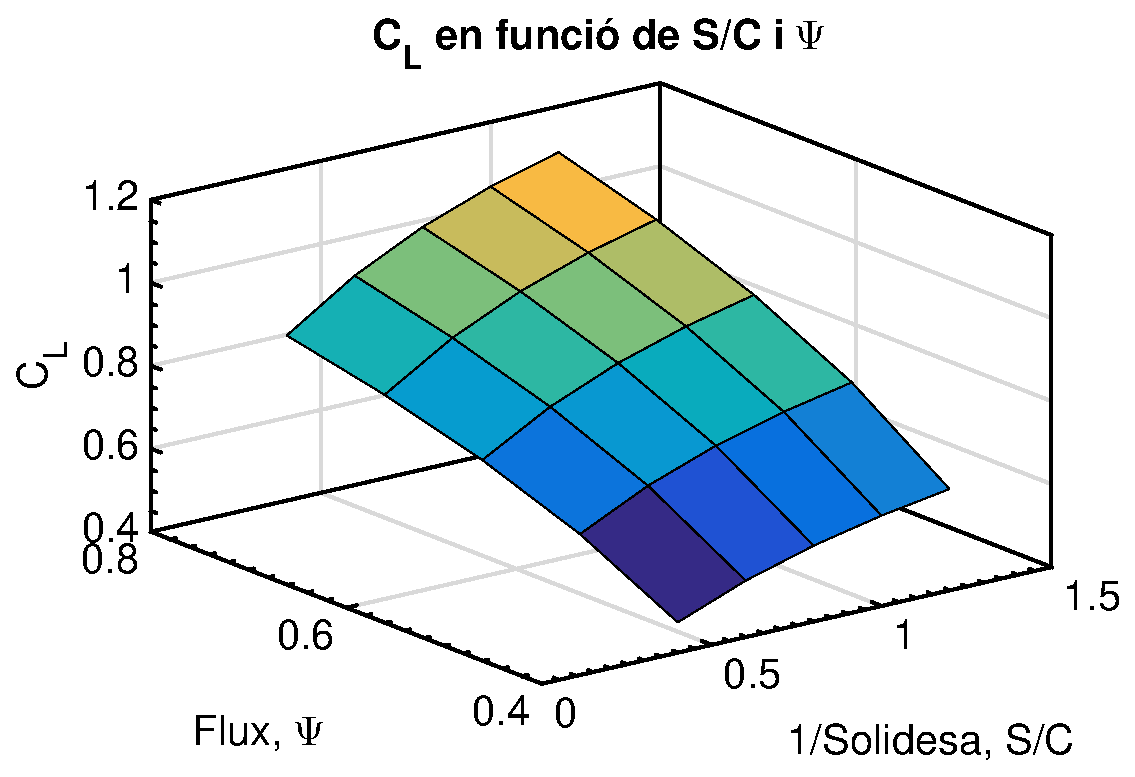
\includegraphics[width=0.8\textwidth]{./code/figures/parametres/CL}
	\caption{Valors de $C_L$ en funció de $S/C$ i $\Psi$.}
	\label{CL}
\end{figure}


\begin{figure}[H]
	\centering
	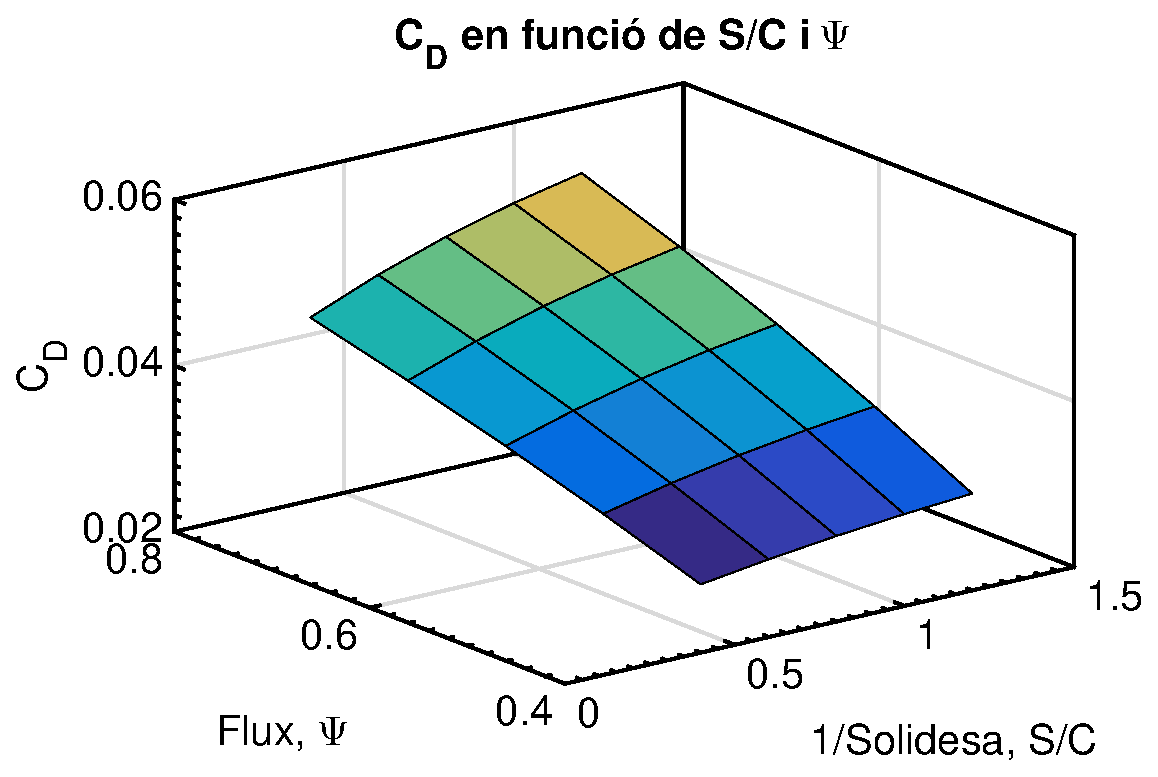
\includegraphics[width=0.8\textwidth]{./code/figures/parametres/CD}
	\caption{Valors de $C_D$ en funció de $S/C$ i $\Psi$.}
	\label{CD}
\end{figure}


\subsection{Càlcul del rendiment de l'esglaó en funció de $S/C$ i $\Psi$}
Els objectius que busquem son: 
\begin{itemize}
\item Mínim nombre d'esglaons possibles per tal de disminuir el pes i volum del compressor.
\item Rendiment adiabàtic bo.
\item Menor àrea frontal possible.
\end{itemize}
Es defineix el rendiment com:
\begin{equation}
\eta_{esg}=\frac{T_{ct}'-T_{0t}}{T_{ct}-T_{0t}}
\end{equation}
On $T_{ct}'$ es la temperatura a la sortida de l'etapa del compressor ideal i $T_{ct}$ la real. Aquest rendiment es pot re-escriure com:
\begin{equation}
\eta_{esg}=1-\frac{T_{it}-T_{bt}'}{T_{ct}-T_{0t}}-\frac{T_{bt}'-T_{ct}'}{T_{ct}-T_{0t}}
\end{equation}
Es a dir, a 1 se li resten les pèrdues del rotor i les pèrdues de l'estator. Relacionant les temperatures amb pressions mitjançant el coeficient $\gamma$:
\begin{equation}
\eta_{esg}=\frac{\bigtriangleup P_{r}+\bigtriangleup P_{e}}{\rho\tau_{esg}}
\end{equation}
Considerant que el grau de reacció es 0.5, la variació de pressió al rotor i a l'estator es la mateixa i per tant: 
\begin{equation}
\eta_{esg}=\frac{\bigtriangleup P_t}{\rho\tau_{esg}}
\end{equation}
Considerant les següents equacions: 
\begin{equation}
\bigtriangleup P_t=\frac{C_D\frac{1}{2}\rho\omega_m^2}{\frac{S}{C}\cos\beta_m}
\end{equation}
\begin{equation}
\tau_{esg}=U(V_{\theta_b}-V_{\theta_a})
\end{equation}
\begin{equation}
R=0.5=\Psi\tan\beta_m
\end{equation}
S'arriba a les següents expressions per al calcul del rendiment: 
\begin{equation}
\tau_{esg}=1-\frac{C_D}{C_{Li}}\Big( 2\Psi+\frac{1}{2\Psi}\Big)
\end{equation}
\begin{equation}
\tau_{23}=1-N\frac{C_D}{C_{Li}}\Big( 2\Psi+\frac{1}{2\Psi}\Big)
\end{equation}
Essent $N$ el nombre d'esglaons del compressor. $C_{Li}$ s'ha definit com: 
\begin{equation}
C_{Li}=\frac{2}{\sigma}(\tan\beta_a-\tan\beta_b)\cos\beta_m
\end{equation}
Finalment, el rendiment per esglaó es pot apreciar a la Figura \ref{ETAesg}. El rendiment total es podrà calcular un cop s'obtingui el nombre d'esglaons que tindrà el compressor. 
\begin{figure}[H]
	\centering
	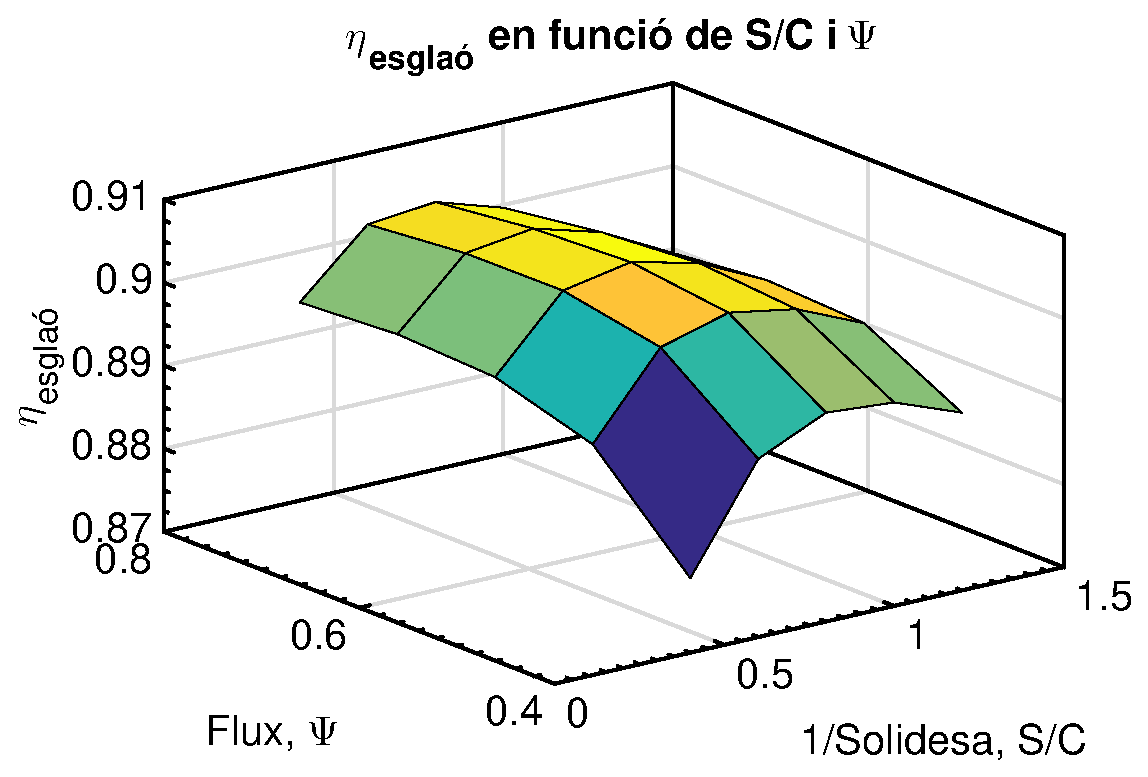
\includegraphics[width=0.8\textwidth]{./code/figures/parametres/ETAesg}
	\caption{Valors de $\eta_{esg}$ en funció de $S/C$ i $\Psi$.}
	\label{ETAesg}
\end{figure}

\subsection{Velocitat axial en funció de $S/C$ i $\Psi$}
La velocitat axial presenta una limitació en el disseny del compressor, ja que no interessa que hagi flux sònic a cap punt del perfil evitant així efectes de compressibilitat. Amb l'objectiu d'evitar aquest fenomen, es limita el número a 0.8. La velocitat axial es troba utilitzant la següent expressió: 
\begin{equation}
V_z=\sqrt{\frac{M^2\gamma R T_{at}}{\frac{1}{(\cos\beta_a)^2}+\frac{M^2\gamma R}{2C_P(\cos\beta_b)^2}}}
\end{equation} 
\begin{figure}[H]
	\centering
	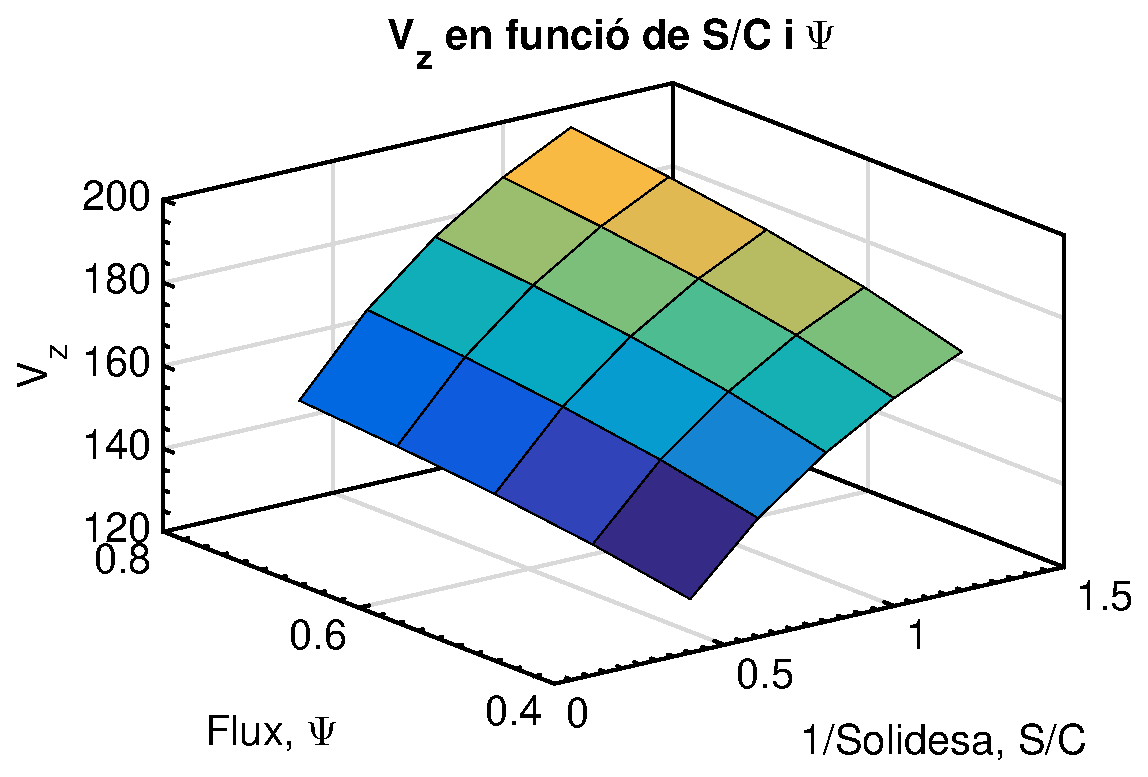
\includegraphics[width=0.8\textwidth]{./code/figures/parametres/Vz}
	\caption{Valors de $V_z$ en funció de $S/C$ i $\Psi$.}
	\label{Vz}
\end{figure}
La velocitat axial haurà d'estar entre els valors de $150m/s$ i $180m/s$. Per sota d'aquests valors el treball aportat per un esglaó es molt baix i per sobre podria donar pas a problemes de combustió. Es verificarà que la velocitat axial estigui entre aquests valors. 
\subsection{Càlcul de la velocitat tangencial en funció de $S/C$ i $\Psi$}
Un cop obtinguda la velocitat axial, calcular la velocitat tangencial es senzill degut a que estan directament relacionades mitjançant el paràmetre de flux. 
\begin{equation}
\Psi=\frac{V_z}{U}
\end{equation}
La velocitat tangencial, o velocitat d'arrossegament, també ha d'estar limitada degut a les càrregues centrífugues que produeix. Per aquesta raó, es verificarà que no sobrepassi el valor de $320m/s$.
\begin{figure}[H]
	\centering
	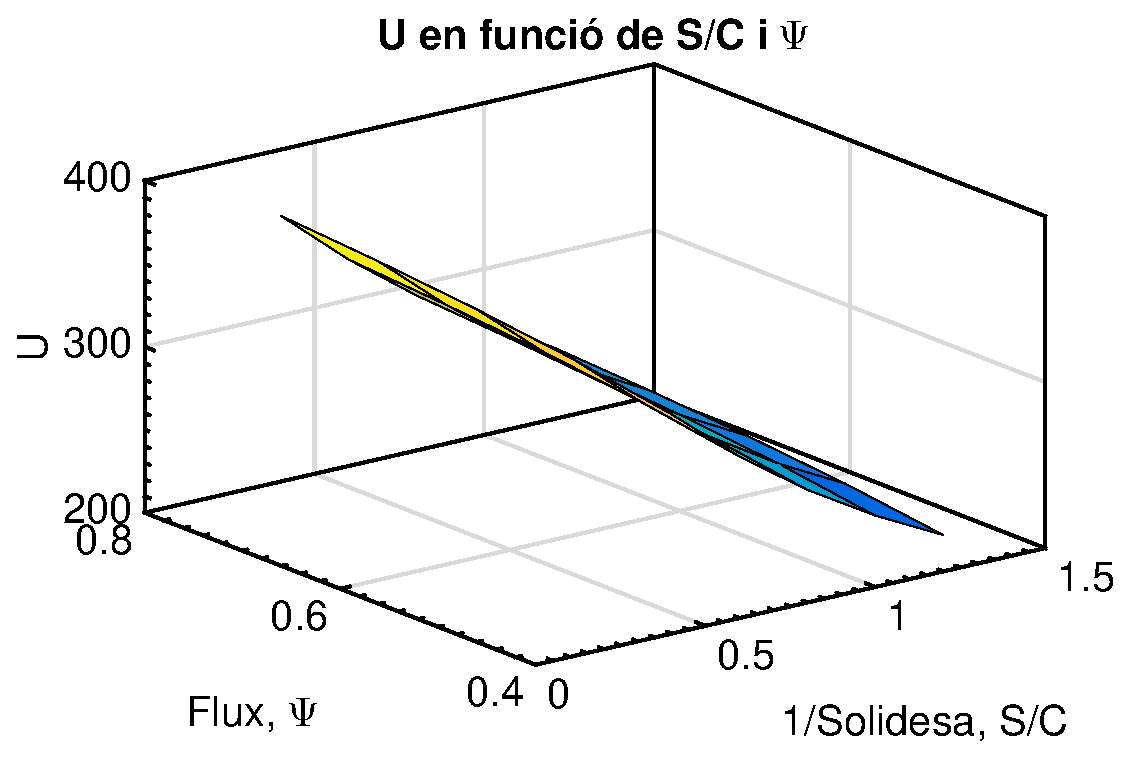
\includegraphics[width=0.8\textwidth]{./code/figures/parametres/U}
	\caption{Valors de $U$ en funció de $S/C$ i $\Psi$.}
	\label{U}
\end{figure}

\subsection{Càlcul del treball de l'esglaó en funció de $S/C$ i $\Psi$}
El treball per esglaó es calcula utilitzant:
\begin{equation}
\tau_{esg}=UV_z(\tan\beta_a-\tan\beta_b)
\end{equation}
\begin{figure}[H]
	\centering
	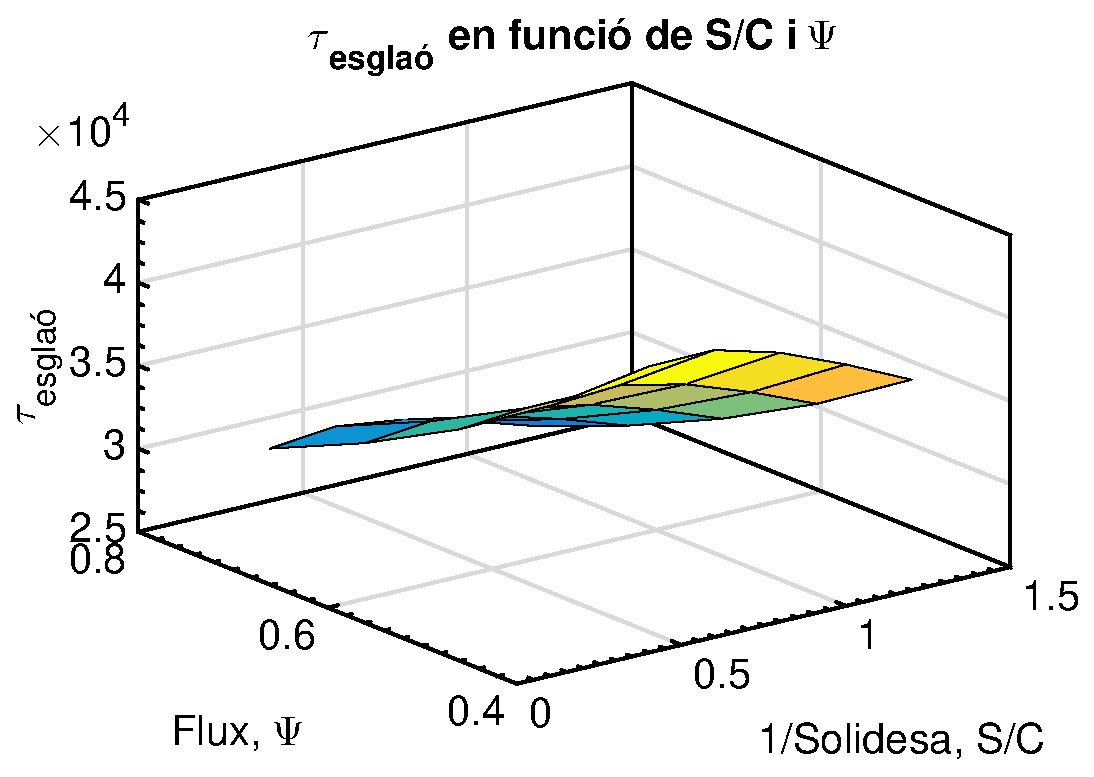
\includegraphics[width=0.8\textwidth]{./code/figures/parametres/TAUesg}
	\caption{Valors de $\tau_{esg}$ en funció de $S/C$ i $\Psi$.}
	\label{TAUesg}
\end{figure}

\subsection{Càlcul de la relació de radis en funció de $S/C$ i $\Psi$}
Es busca calcular al relació entre els radis exterior i interior de l'àlep. Per tal de trobar-la, es necessari realitzar un estudi sobre els esforços centrífugs. Es considerarà que l'àlep te una forma cilíndrica. Com que aquesta suposició no es real, s'haurà d'incorporar el següent factor:
\begin{equation}
\lambda=\frac{\sigma_{real}}{\sigma_{cilindre}}
\end{equation}
El valor de $\lambda$ oscil·la entre $0.6$ y $0.8$. En aquest disseny es prendrà $\lambda=0.7$.
La força centrífuga es pot calcular com: 
\begin{equation}
F_c=\int_{r_i}^{r_e} A(r)\rho\omega^2rdr
\end{equation}
L'esforç a un àlep es: 
\begin{equation}
\sigma=\frac{\rho\omega^2}{A}\int_{r_i}^{r_e} A(r)rdr
\end{equation}
Tenint en compte la consideració ja mencionada d'assimilar l'àlep a un geometria cilíndrica amb àrea constant: 
\begin{equation}
\sigma_{cilindre}=\rho\omega^2\frac{r_e^2-r_i^2}{2}
\end{equation}
Aplicant el factor de correcció $\lambda$:
\begin{equation}
\sigma_{real}=\lambda\rho\omega^2\frac{r_e^2-r_i^2}{2}
\end{equation}
Operant amb els valors coneguts fins ara es pot arribar a l'expressió: 
\begin{equation}
\frac{r_i}{r_e}=\frac{U^2-\frac{\sigma}{2\lambda\rho}}{U^2+\frac{\sigma}{2\lambda\rho}}
\label{rireeq}
\end{equation}
Amb l'objectiu d'incorporar un factor de seguretat: 
\begin{equation}
\sigma=\frac{\sigma_{max}}{4}
\end{equation}
Els valors de $\sigma_{max}$ i de densitat estan definits pel material utilitzat per a construir aquesta primera etapa. Es considera que el material serà un aliatge d'alumini: L-316. Les seves característiques son: 
\begin{equation}
\nonumber \sigma_{max}=39·10^6 kg/m^2
\end{equation}
\begin{equation}
\nonumber \rho=2.8 kg/dm^2
\end{equation}
\begin{figure}[H]
	\centering
	\includegraphics[width=0.8\textwidth]{./code/figures/parametres/rire}
	\caption{Valors de $r_i/r_e$ en funció de $S/C$ i $\Psi$.}
	\label{rire}
\end{figure}

\subsection{Càlcul del radi exterior, radi interior, radi mitjà i altura en funció de $S/C$ i $\Psi$}
Es calcula el radi exterior utilitzant la següent expressió del flux màssic (consum, G) al compressor: 
\begin{equation}
G=2\rho V_z\pi\Big(\frac{r_e^2-r_i^2}{2}\Big)
\end{equation}
Aïllant es pot obtenir: 
\begin{equation}
r_e=\sqrt{\frac{G}{\pi\Big(1-\frac{r_i^2}{r_e^2}\Big)V_z\rho_{at}}}
\end{equation}
Un cop obtingut el valor del radi exterior, el radi interior es pot calcular amb l'expressió \ref{rireeq}. L'altura dels àleps es la diferencia entre el radi exterior i el radi interior: 
\begin{equation}
h=r_e-r_i
\end{equation}
Els valors obtinguts son els següents: 
\begin{figure}[H]
	\centering
	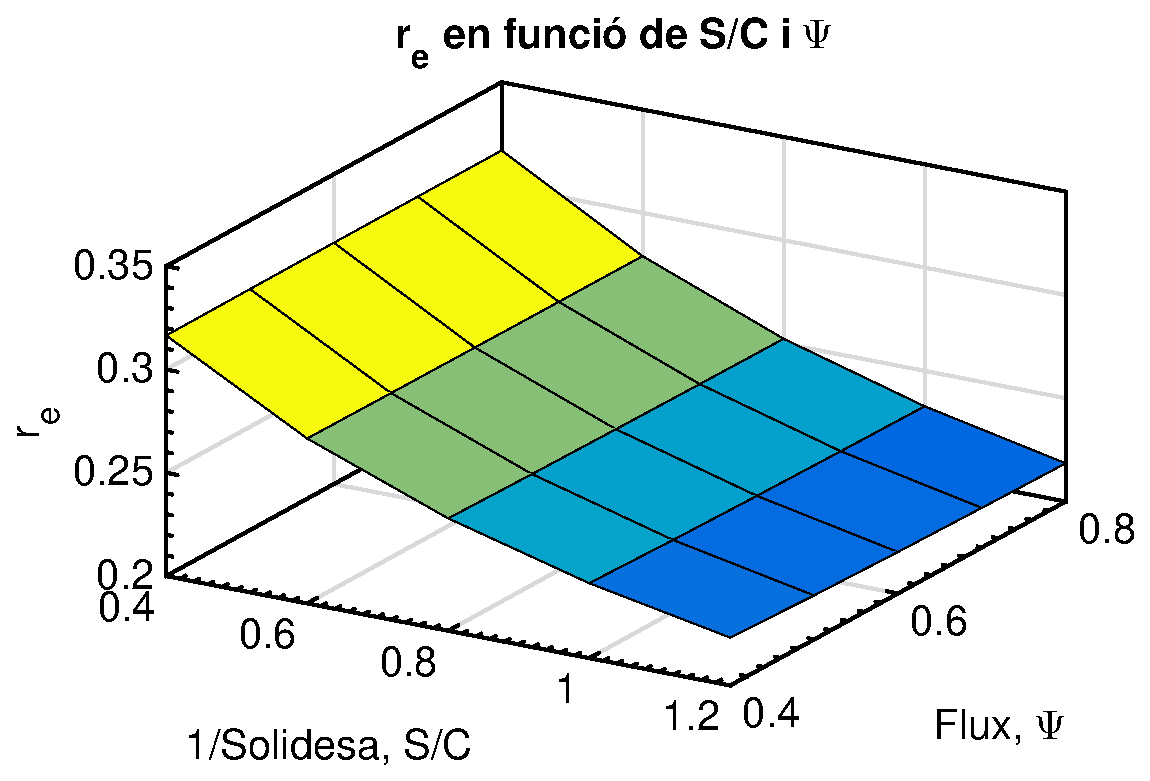
\includegraphics[width=0.8\textwidth]{./code/figures/parametres/re}
	\caption{Valors de $r_e$ en funció de $S/C$ i $\Psi$.}
	\label{re}
\end{figure}


\begin{figure}[H]
	\centering
	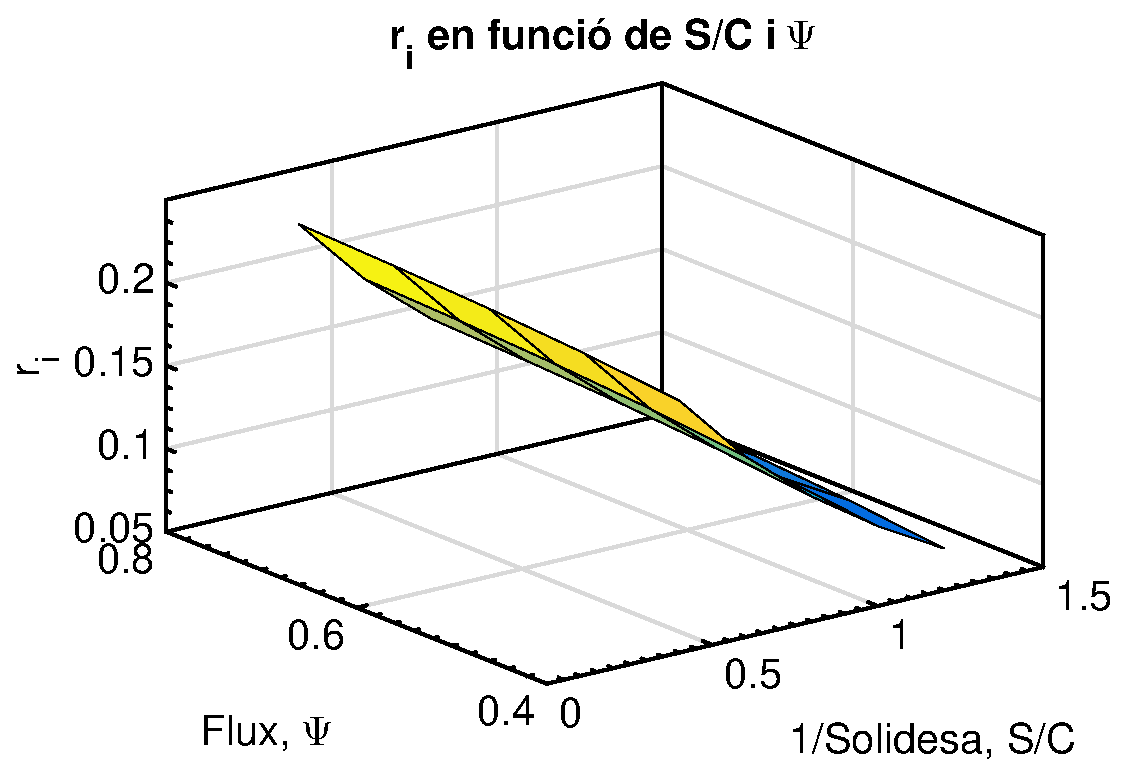
\includegraphics[width=0.8\textwidth]{./code/figures/parametres/ri}
	\caption{Valors de $r_i$ en funció de $S/C$ i $\Psi$.}
	\label{ri}
\end{figure}


\begin{figure}[H]
	\centering
	\includegraphics[width=0.8\textwidth]{./code/figures/parametres/rm}
	\caption{Valors de $r_m$ en funció de $S/C$ i $\Psi$.}
	\label{rm}
\end{figure}

\begin{figure}[H]
	\centering
	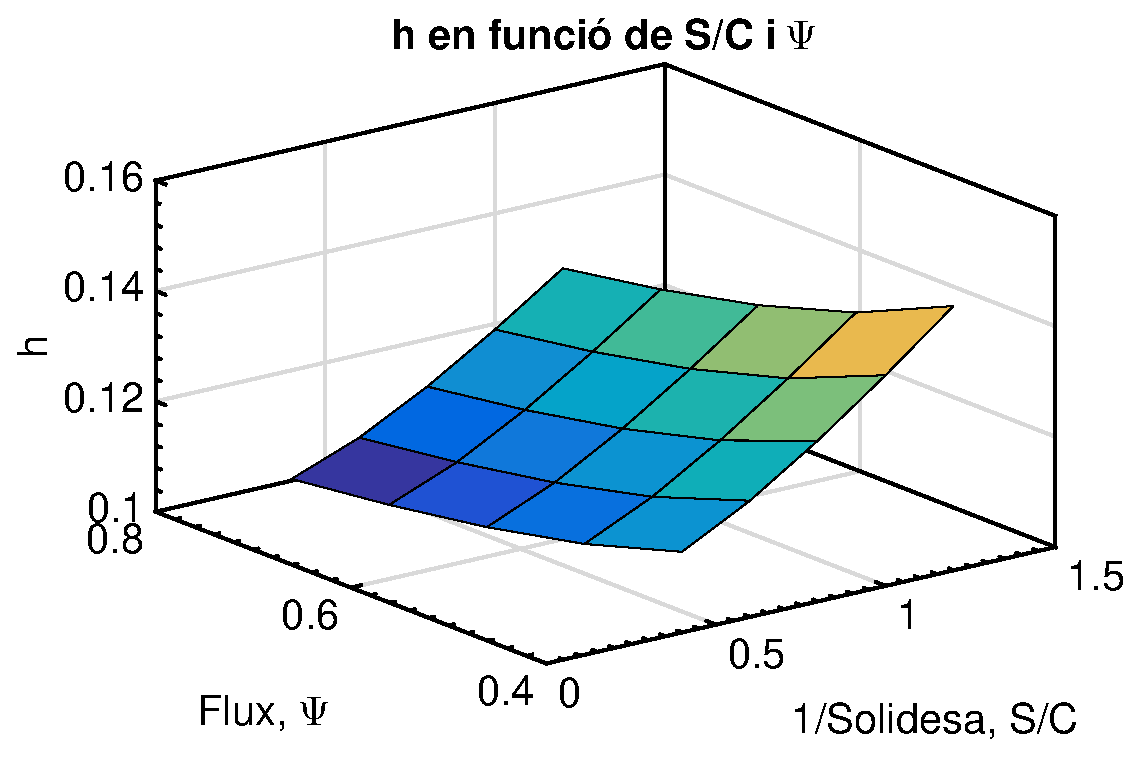
\includegraphics[width=0.8\textwidth]{./code/figures/parametres/h}
	\caption{Valors de $h$ en funció de $S/C$ i $\Psi$.}
	\label{h}
\end{figure}

\subsection{Càlcul de la velocitat de gir en funció de $S/C$ i $\Psi$}
Per últim, es calcula la velocitat de gir del rotor. Aquesta es: 
\begin{equation}
N(rpm)=\frac{60U}{2\pi r_m}
\end{equation}

\begin{figure}[H]
	\centering
	\includegraphics[width=0.8\textwidth]{./code/figures/parametres/RPM}
	\caption{Valors de $N$ en funció de $S/C$ i $\Psi$.}
	\label{RPM}
\end{figure}
\clearpage
\section{Elecció de paràmetres $S/C$ i $\Psi$}
Es parteix del coneixement que el treball específic que ha de subministrar el nostre motor és $\tau_{23} = 300000 J/kg$.\\

A partir de motors similars, s'aprecia que les solucions per compressors estan entre 7, 8, 9 i 10 graons. Per tant, per cada un dels 4 casos es pot trobar el valor que es tindria de solidesa i el coeficient de flux del gràfic de $\tau_{esc}$. S'escollirà el cas que tingui un major rendiment per escaló de tots els possibles. \\

Primer de tot es necessari saber el treball específic que ha de realitzar cada etapa de compressió segons el numero total d'etapes. Es calcula com $\tau_{esc}=\tau_{23}/N$ on $N$ és el número d'etapes de compressió.

\begin{longtable}[H]{C{1.5cm} C{2.5cm}}
	\toprule[2pt]
	\textbf{N} &  \textbf{$\tau_{esc} \quad [J/kg]$} \\ \bottomrule[2pt]
	7 & $4.29\mathrm{x}10^4$\\ \midrule
	8 & $3.75\mathrm{x}10^4$\\ \midrule
	9 & $3.33\mathrm{x}10^4$\\ \midrule
	10&$3.00\mathrm{x}10^4$
	\\ \bottomrule[2pt]
	\caption{Treball específic segons etapes de compressió}
	\label{valorsI}
\end{longtable}

Després, es superposen (Figura \ref{TAUS}) els resultats obtinguts per cada escaló segons nombre d'etapes amb els valors de $\tau$ inicialment calculats per diferents $S/C$ i $\Psi$.\\
\begin{figure}[H]
	\centering
	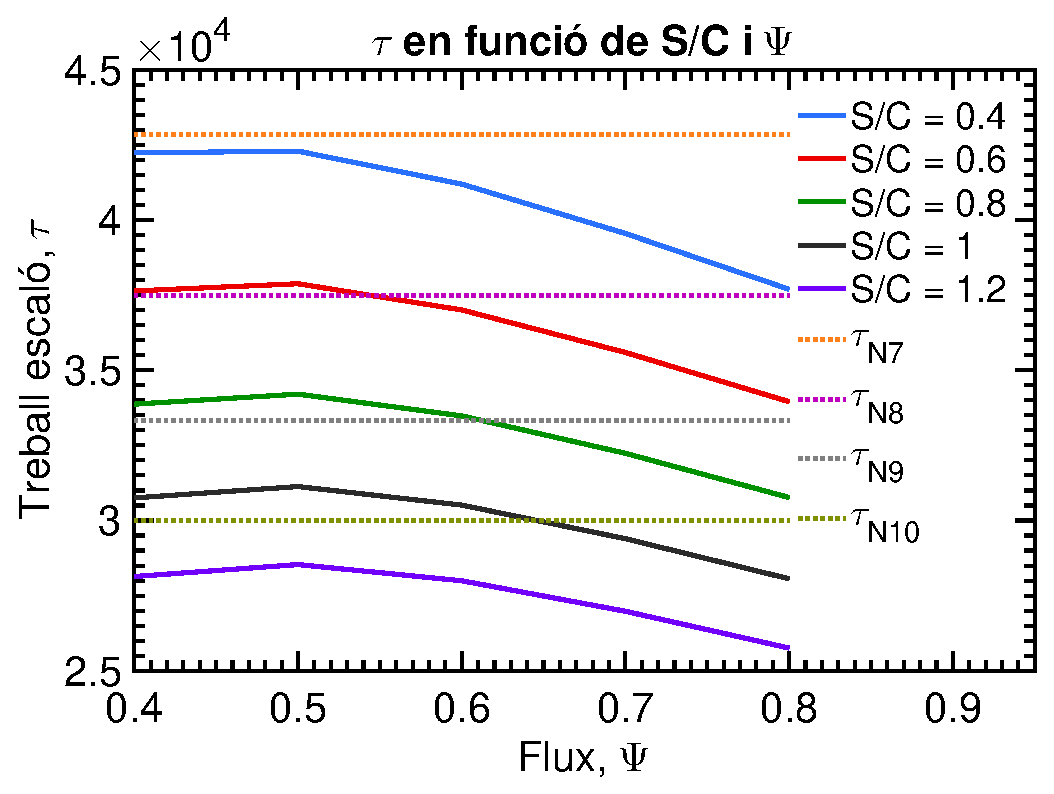
\includegraphics[width=0.8\textwidth]{./code/figures/parametres/TAUSesg.eps}
	\caption{Valors de $\tau$ en funció de $S/C$ i $\Psi$.}
	\label{TAUS}
\end{figure}
\clearpage

Es busca l'intersecció dels treballs específics calculats per a cada etapa amb els treballs d'escaló calculats per per diferents valors de $S/C$ i $\Psi$.

El resultat, permet veure quin paràmetre $S/C$ es el millor per a cada punt d'intersecció, però per saber el flux ($\Psi$) caldrà interpolar entre els dos punts més propers a l'intersecció.\\

S'han interpolat els valors del flux ($\Psi$) linealment a partir de dos punts d'informació propers a l'intersecció, $(x_a,y_a)$ i $(x_b,y_b)$, per obtenir un tercer punt interpolat $(x,y)$ segons,
\begin{equation}
	y = y_a + (x-x_a)\frac{(y_b-y_a)}{(x_b-x_a)}
\end{equation}
per aquest cas particular,
\begin{equation}
\Psi_N = \Psi_a + (\tau_{N}-\tau_a)\frac{(\Psi_b-\Psi_a)}{(\tau_b-\tau_a)}
\end{equation}

Aquesta aproximació lineal, és vàlida ja que es treballa en un interval petit entre les dues dades conegudes. Finalment, els resultats obtinguts apareixen agrupats a la Taula \ref{paramIni}.

\begin{longtable}[H]{C{1.5cm} C{1.5cm} C{1.5cm}}
	\toprule[2pt]
	\textbf{N} &  \textbf{$S/C$}  & \textbf{$\Psi$}\\ \bottomrule[2pt]
	7 & -- & --\\ \midrule
	8 & 0.6 &0.5437\\ \midrule
	9 & 0.8 &0.6121\\ \midrule
	10 & 1 &0.6455
	\\ \bottomrule[2pt]
	\caption{Paràmetres escollits inicialment}
	\label{paramIni}
\end{longtable}

\subsection{Selecció del cas amb major rendiment}
\begin{figure}[H]
	\centering
	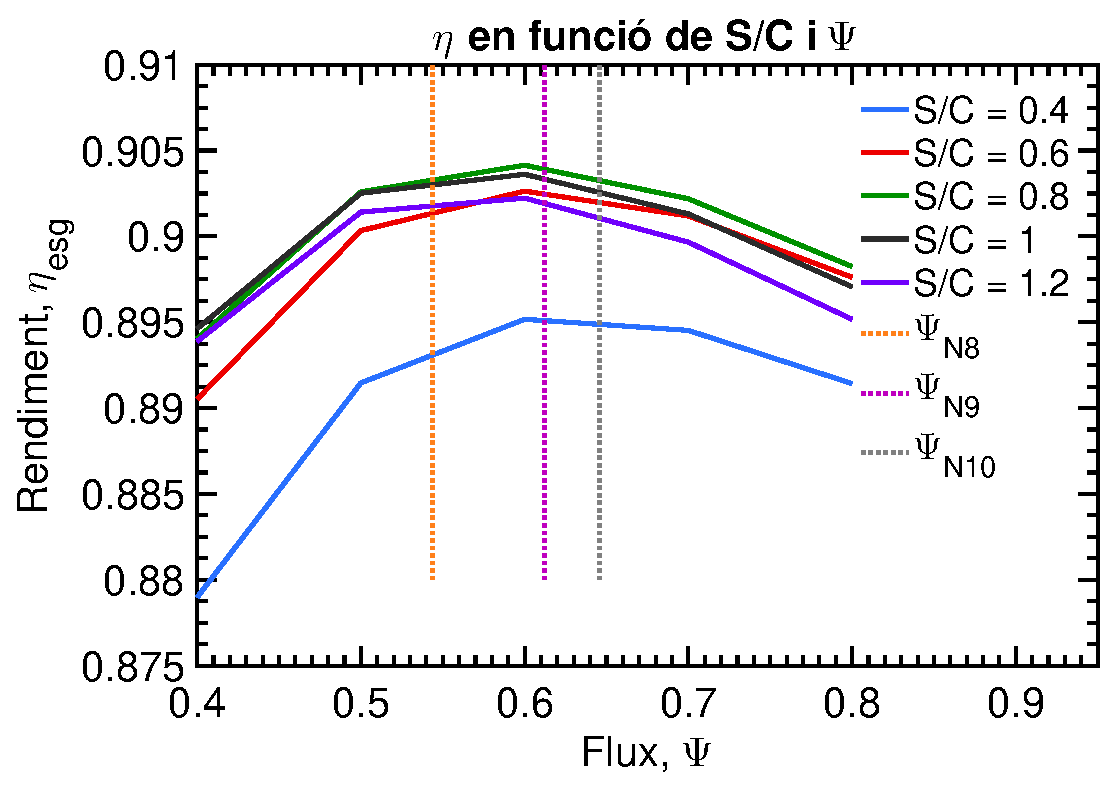
\includegraphics[width=0.8\textwidth]{./code/figures/parametres/FLUXs}
	\caption{Valors de $\eta$ en funció de $S/C$ i $\Psi$.}
	\label{FLUXs}
\end{figure}
Un cop se saben els paràmetres $S/C$ i $\Psi$, per trobar els rendiments associats, se superposen els valors de $\eta$ en funció de $S/C$ i $\Psi$ calculats amb anterioritat amb els valors de $\Psi$ de la Taula \ref{paramIni}. Aquest procés està il·lustrat a la Figura \ref{FLUXs}.\\

A l'igual que el primer cas, ara s'interpola el valor de $\eta$ entre els dos punts més pròxims a l'intersecció. Obtenint-se els resultats de la Taula \ref{paramEta}
\begin{longtable}[H]{C{1.5cm} C{1.5cm} C{1.5cm} C{1.5cm}}
	\toprule[2pt]
	\textbf{N} &  \textbf{$S/C$}  & \textbf{$\Psi$}& \textbf{$\eta_{esc}$}\\ \bottomrule[2pt]
	7 & -- & -- & --\\ \midrule
	8 & 0.6 &0.5437 & 0.9013 \\ \midrule
	9 & 0.8 &0.6121 & 0.9039\\ \midrule
	10 & 1 &0.6455& 0.9026
	\\ \bottomrule[2pt]
	\caption{Paràmetres escollits inicialment, més $\eta_{esc}$}
	\label{paramEta}
\end{longtable}

La primera impressió, es de que el compressor de 9 etapes, té el millor rendiment. Tot i això, és necessari calcular el rendiment total del compressor per veure si és realment així, ja que tots els rendiments tenen valors molt similars entre si.\\

A partir de l'equació \ref{eq23} es pot calcular el rendiment total del compressor. Per fer-ho, com en els anteriors casos, es necessari interpolar els valors de $C_D$ i $C_{Li}$, seguint el mateix principi.

\begin{equation}
	\eta_{23} = 1-N\frac{C_D}{C_{Li}}\Big(2\Psi+\frac{1}{2\Psi}\Big)
	\label{eq23}
\end{equation}

\begin{longtable}[H]{C{1.5cm} C{1.5cm} C{1.5cm} C{1.5cm}}
	\toprule[2pt]
	\textbf{N} &  \textbf{$S/C$}  & \textbf{$\Psi$}& \textbf{$\eta_{23}$}\\ \bottomrule[2pt]
	7 & -- & -- & --\\ \midrule
	8 & 0.6 &0.5437 & 0.2142 \\ \midrule
	9 & 0.8 &0.6121 & 0.1360\\ \midrule
	10 & 1 &0.6455& 0.0278
	\\ \bottomrule[2pt]
	\caption{Paràmetres escollits inicialment, més $\eta_{23}$}
	\label{paramEta23}
\end{longtable}
Els resultats obtinguts són molt interessants, ja que mostren que el compressor més eficient és el de 8 etapes, per tant, els paràmetres escollits són:
\begin{longtable}[H]{C{1.5cm} C{1.5cm} C{1.5cm}}
	\toprule[2pt]
	\textbf{N} &  \textbf{$S/C$}  & \textbf{$\Psi$}\\ \bottomrule[2pt]
	8 & 0.6 &0.5437\\ \bottomrule[2pt]
	\caption{Paràmetres escollits}
	\label{param}
\end{longtable}
\clearpage
\section{Opcional 1. Càlcul de $S$ i $N$ (número d'àleps al primer graó)}
\label{op1}
Els dos apartats opcionals s'han resolt amb el codi adjunt titulat \textit{opcional.m} pel cas escollit de 8 etapes. Així, un cop \textbf{S/C} s'ha triat (0.6) i es tenen calculades les alçades de la primera etapa, caldrà fixar el paràmetre $\frac{c}{h}$ per tal de poder trobar el pas i el número d'àleps. A classe es va recomanar el següent valor de $\frac{c}{h}$ :
\begin{equation}
\frac{c}{h} = \frac{1}{2.5}
\end{equation}
Doncs bé, com es volen trobar tots els àleps del primer graó caldrà trobar els del rotor i els del estator. Per això es necessita conèixer l'alçada de les seccions \textit{1a, 1b, 2c} doncs així:
\begin{multicols}{2}
  \begin{equation}
    h_{rotor} = \frac{h_{1a}+h_{1b}}{2} = 0.1121m
  \end{equation}\break
  \begin{equation}
    h_{estator} = \frac{h_{1b}+h_{2a}}{2} = 0.1085m
  \end{equation}
\end{multicols}
La forma en la que s'han calculat les alçades a les seccions 1b i 2c es detalla a l'apartat \ref{op2}.
Així:
\begin{multicols}{2}
  \begin{equation}
    S_{rotor} = \frac{S}{C}\times h_{rotor} = 0.067
  \end{equation}\break
  \begin{equation}
    S_{estator} = \frac{S}{C}\times h_{estator} = 0.065
  \end{equation}
\end{multicols}
Per últim, cal parlar de quin és el valor de $r_m$. Pel cas de 8 etapes ha donat que:
\begin{equation}
r_m = 0.2221m
\end{equation}
Amb aquests valors la troba  del número d'àleps és immediata. Es dividirà el perímetre circular delimitat pel radi mig entre la separació entre àleps, és a dir, el pas o \textbf{\textit{S}}. S'arrodonirà a número enter per truncament.
\begin{equation}
N = \frac{2\pi r_m}{S}
\end{equation}
Obtenint així:
\begin{longtable}[H]{C{2.5cm} C{2.5cm}}
	\toprule[2pt]
	\textbf{Secció} &  \textbf{N} \\ \bottomrule[2pt]
	Rotor & 51\\ \midrule
	Estator & 53\\ \midrule
	\textbf{Etapa 1} & 104\\
	\bottomrule[2pt]
	\caption{Àleps del primer graó}
	\label{aleps}
\end{longtable}
\section{Opcional 2. Càlcul de la longitud total del compressor}
\label{op2}
Per aquest apartat, cal conèixer la distribució de cordes al llarg de les diferents etapes del compressor.
Per donar un exemple, la longitud de la primera etapa es calcularia de la següent manera:
\begin{align}
\label{eqL}
\begin{split}
L_{stage_I} = L_{IGV} + L_{d_{RI}} + L_{P_{RI}} + L_{d_{EI}} +  L_{P_{EI}}  \\
L_{stage_I} = 1.24C_{R} + 0.4C_{RI} + C_{RI}\cos{\beta_m} + 0.25C_{EI} + C_{EI}\cos{\beta_m}
\end{split}
\end{align}
S'anirien sumant les vuit etapes per obtenir així la longitud total del compressor. Igual que l'anterior apartat, aquest s'ha realitzat amb el codi adjunt titulat \textit{opcional.m}.

A l'equació \ref{eqL} es veu clarament que cal conèixer $\beta_m$ així com la distribució de les cordes a cada etapa. Doncs bé, per començar s'ha definit la distribució del paràmetre $\frac{c}{h}$. Ja es va dir a l'apartat \ref{op1} que $\Big(\frac{c}{h}\Big)_I = \frac{1}{2.5}$. Així, per calcular la longitud total s'estableix que:
\begin{equation}
\Big(\frac{c}{h}\Big)_N = 1.25\Big(\frac{c}{h}\Big)_I
\end{equation}
On N indica l'etapa final en aquest cas.

Per tant, conegut el paràmetre $\frac{c}{h}$ a cada secció cal calcular finalment el valor de les alçades a cada secció. Per fer això, és necessari trobar la distribució de pressions, temperatures i conseqüentment, de densitats. Amb la finalitat de trobar aquests valors, s'han fet les següents hipòtesis:

\begin{itemize}
\item $r_m$ constant.
\item Repetició de la geometria d'hileres per etapa ($\alpha_1 = \beta_2 = \alpha_3$)
\item $\pi_{ab} = \pi_{ac}$
\item $V_z$ constant.
\item $\Psi$ constant.
\end{itemize}

Fent aquestes hipòtesis, s'empra el triangle de velocitats que permet propagar les condicions de pressió i temperatura a l'entrada del compressor per tota la resta, coneixent també el treball per esglaó i el rati de compressió per etapa.
\begin{equation}
W_{esg} = \frac{W_{total}}{etapes} = \frac{300000}{8} J/Kg
\end{equation}
\begin{equation}
\frac{P_b}{P_a} = 1 + \frac{1}{2}\gamma CpM_{ra}^2
\end{equation}
On Cp representa el coeficient de pressió estàtica \footnote{Tant per la definició del coeficient de pressió estàtica com per la 4a hipòtesis, es suposa flux incompressible.}
\begin{equation}
Cp = 1 - \Big( \frac{\cos{\beta_A}}{\cos{\beta_B}} \Big)^2
\end{equation}
Així doncs, la metodologia de càlcul iterativa que s'ha seguit es la següent:
\begin{enumerate}
\item Passar pressions i temperatures totals de la secció $a_i$ a estàtiques.
\item Trobar la densitat a la secció $a_i$.
\item Propagar pressions i temperatures totals a la secció $b_i$ amb $W_{esg}$ per les temperatures i amb $\pi_{ba}$ per les pressions.
\item Emprar triangle de velocitats amb les hipòtesis abans marcades, per trobar així $V_b$.
\item Passar pressions i temperatures totals de la secció $b_i$ a estàtiques.
\item Trobar la densitat a la secció $b_i$.
\item Trobar $h_{rotor}$ i $h_{estator}$ d'etapa.
\item Per la secció $a_{i+a}$ suposar la mateixa temperatura total que a secció $b_i$ així com la mateixa $V_a$.
\end{enumerate}
Els càlculs es poden veure en tot detall al codi adjunt anomenant \textit{opcional.m}.
Finalment, s'han obtingut els següent resultats:
\begin{figure}[H]
	\centering
	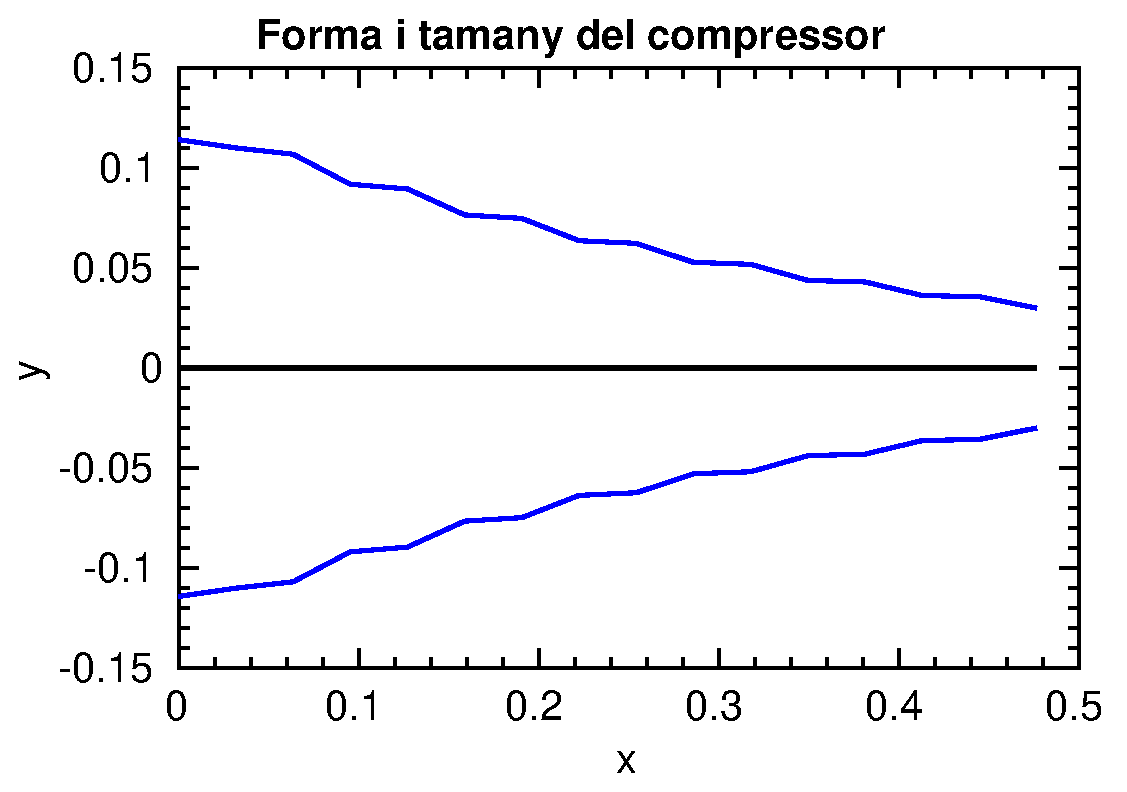
\includegraphics[width=0.8\textwidth]{./code/figures/parametres/compressor_shape.eps}
	\caption{Tamany del compressor}
	\label{shape}
\end{figure}
Realment el compressor no tindria aquesta forma doncs al seu interior la part central aniria creixent de diàmetre. No obstant, l'àrea anular seria la mateixa.
\begin{longtable}[H]{C{5cm} C{2.5cm}}
	\toprule[2pt]
	Longitud del compressor &  \textbf{0.48m} \\ \bottomrule[2pt]
	\caption{Longitud del compressor}
	\label{aleps}
\end{longtable}
Les files de les tres taules següents representen les successives etapes del compressor.
\begin{figure}[H]
	\centering
	\begin{large}\begin{tabular}{|c|c|}
\hline
$h_a$&$h_b$\\\hline
0.11&0.11\\\hline
0.11&0.09\\\hline
0.09&0.08\\\hline
0.07&0.06\\\hline
0.06&0.05\\\hline
0.05&0.04\\\hline
0.04&0.04\\\hline
0.04&0.03\\\hline
\end{tabular}
\end{large}
	\caption{Alçades [m]}
\end{figure}
\begin{figure}[H]
	\centering
	\begin{large}\begin{tabular}{|c|c|c|c|}
\hline
$T_a$&$T_b$&$Tt_a$&$Tt_b$\\\hline
255.32&285.94&288.00&325.35\\\hline
292.68&323.29&325.35&362.70\\\hline
330.03&360.64&362.70&400.05\\\hline
367.38&397.99&400.05&437.40\\\hline
404.73&435.34&437.40&474.75\\\hline
442.08&472.69&474.75&512.10\\\hline
479.43&510.04&512.10&549.45\\\hline
516.78&547.39&549.45&586.80\\\hline
\end{tabular}
\end{large}
	\caption{Temperatures [K]}
\end{figure}
\begin{figure}[H]
	\centering
	\begin{large}\begin{tabular}{|c|c|c|c|}
\hline
$P_a$&$P_b$&$Pt_a$&$Pt_b$\\\hline
64355.72&77586.81&98100.00&121914.41\\\hline
84174.52&125887.48&151509.92&188289.94\\\hline
135309.45&202281.93&233998.54&290803.20\\\hline
215817.24&322736.10&361397.55&449129.15\\\hline
342262.07&512171.65&558158.16&693654.66\\\hline
540449.00&809451.55&862043.82&1071310.54\\\hline
850548.03&1275127.13&1331378.10&1654578.75\\\hline
1335047.53&2003470.97&2056238.46&2555403.65\\\hline
\end{tabular}
\end{large}
	\caption{Pressions [Pa]}
\end{figure}

Després d'analitzar tots els resultats, es creu que donen uns valors lògics que segueixen la mateixa tendència que els mostrats al \textit{Mattingly [Secció 9-4]}. És evident que les hipòtesis introduïdes generen un error. No obstant, són molt útils per obtenir una primera aproximació al disseny un compressor sencer.

\newpage


\newpage
\bibliographystyle{unsrt}
\bibliography{Ingenieria_computacional}
\end{document}
